\documentclass{scrartcl}
\usepackage{my}
\usepackage{subcaption}
\usepackage{biblatex}
\addbibresource{report.bib}

\title{Conformal Prediction}
\author{Satyaki Sen}
\begin{document}
\maketitle

\section{Introduction}
In this document, we will overview some concepts relating to \emph{Conformal Prediction}, 
which is an algorithm for producing prediction sets from a model that are statistically 
guaranteed to contain the true answer with some set probability. In section~\ref{sec:intro}, 
we will introduce the conformal prediction algorithm, and explain how it works. In section~\ref{sec:classification},
we discuss how it is used for classification, and show the results of some experiments we ran. Section~\ref{sec:regression}
shows the applications of conformal prediction to regression models, and in section~\ref{sec:text}, we discuss the approaches
to applying conformal prediction to text generation models, and the results of our experiments on TriviaQA.

\section{What is Conformal Prediction?}
\label{sec:intro}
As Machine Learning models are used more and more, it becomes more important
 that such models are correct in their answers. \emph{Conformal Prediction}
is a method for guaranteeing statistically that a model produce the correct answer with some set probability.
It was introduced by Vovk and collaborators, in \cite{vovkbook}.
Suppose that our model takes in questions, or data points, or whatever it is we care about from some set $X$, 
and produces outputs $y \in Y$; these may be answers to questions, or predictions for regression. The task of 
conformal prediction is to produce prediction sets $S \subset Y$ from the model such that the set $S$ contains 
the true answer with probability at least $1 - \alpha$(here $\alpha$ is some chosen miscoverage threshold). 
Essentially, conformal prediction \footnote{This is really split conformal prediction. We will not deal with the `full' version of conformal prediction here.} 
is the following process, which is explained in \cite{introcp}:

\begin{itemize}
    \item Assign a score $s(x, y)$ to a pair $(x, y) \in X \times Y$. This measures how strange it would be for 
    $y$ to be the true answer for $x$. In fact, we can guarantee coverage \emph{regardless of the choice of $s$}.
    A better score function provides prediction sets that are more useful, but we can guarantee $1 - \alpha$ 
    coverage regardless of what choice we make.

    \item Over some calibration data $\mathcal{D}_{cal}$, which contains object $x \in X$ along with the true 
    values $y \in Y$. Then compute the scores $s(x_i, y_i)$ for $(x_i, y_i) \in \mathcal{D}_{cal}$, and compute the $1 - \alpha$
    quartile of these scores.\footnote{In practice, it is often better to compute the $\lceil (n + 1)(1 - \alpha) \rceil/n$ quartile, but this is a small difference.} 
    That is, the value $\hat{q}$ such that only a fraction $\alpha$ of the scores 
    are higher than $\hat{q}$.

    \item Now, when faced with a new object $x' \in X$, we will include a value $y \in Y$ in the prediction set 
    $\Gamma^{\alpha}(x')$ only if $s(x', y) < \hat{q}$.
    
\end{itemize}

This conformal algorithm works under the assumption that the data we face in practice is \emph{exchangeable}
with the calibration data. This \emph{split conformal prediction} approach is nice for many reasons: we assume little about the distribution of the data
that is encountered, and the approach does not care about any specifics of the model itself. The main factor that 
tell us how useful the prediction sets are is their size, naturally, larger sets are less specific and informative.

\begin{proof}[Proof of the conformal coverage guarantee.]
Sort our $n$ calibration scores as $s_1 < s_2 < \dots < s_n$, so that $\hat{q} = s_{n(1 - \alpha)}$ (it is fine to assume $(1 - \alpha)n$ is an integer). 
Now when we see a new example $x$, we will include $y$, the true label, in the prediction set as long as $s(x, y) \le \hat{q} = s_{n(1 - \alpha)}$. 
By exchangeability, $(x, y)$ will be equally likely to fall at any position within the ordering $s_1 < s_2 < \dots < s_n$. 
Thus, it has a $1 - \alpha$ chance of falling before $s_{n(1 - \alpha)}$, as desired.
\end{proof}

\section{Classification}
\label{sec:classification}
This is all well and good, but how do we actually compute the key ingredients of the above process, 
the non-conformity scores $s(x, y)$?. A natural choice, if we have the probabilities assigned by the model 
to each class in $Y$, is to define the score by $s(x, y) = 1 - p(y)$. Assuming that the probabilities $p(y)$ are
reasonably well associated with how well class $y$ represents object $x$, this satisfies the desired property:  
the more correct classes have lower scores than the ones that do not represent the object. 

\begin{figure}[h]
    \centering
        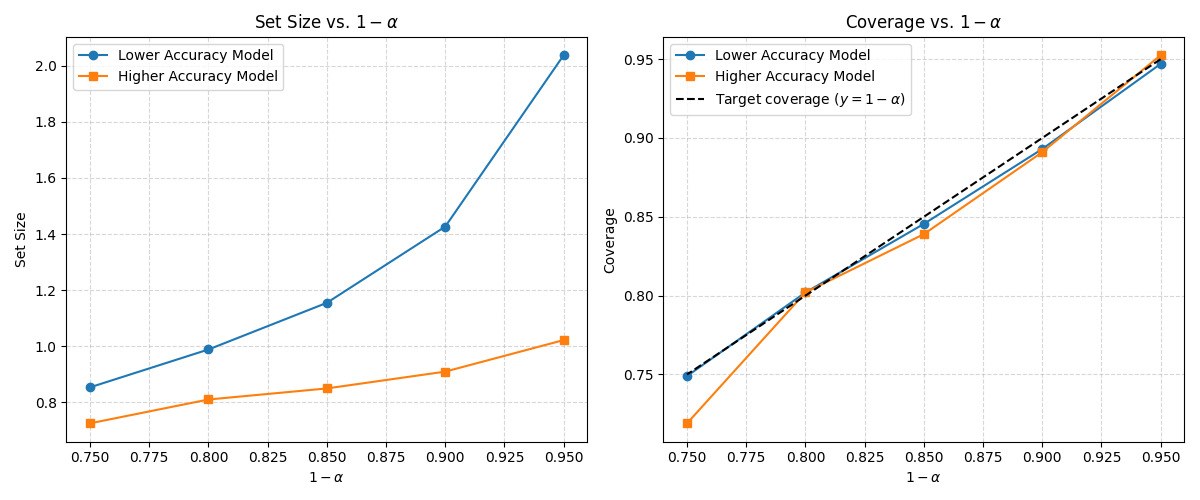
\includegraphics[width=\textwidth]{graphs/conformal_simple_comparison.png}
        \caption{The two models are both MNIST classifiers with 90\% and 95\% accuracy respectively.
        We plot the average set size and empirical coverage for both models.}
    \label{fig:simpleCP-comparison}
\end{figure}

The above Figure~\ref{fig:simpleCP-comparison} demonstrate two characteristics of CP. With a more accurate model, the set sizes can be smaller, 
because there is less uncertainty as to what the true label is. Additionally, the conformal algorithm can also provide
us with size $0$ sets, as evidenced by the average set sizes taking values $< 1$. This is to be expected if request $1 - \alpha$ 
less than the models accuracy, since we do not need to add anything to guarantee coverage. \medskip

One alternative to the simple score function we used above is known as \emph{APS}, for adaptive prediction sets.
Ideally, with APS, the set sizes should more accurately reflect how difficult or easy the classification question is, 
producing larger sets when the model is unsure. Here, we define scores as 
\[ s(x, y) \coloneq \sum_{p(y') \ge p(y)} p(y'), \]
that is, the score is the sum of all the softmax probabilities that are at least the probability of the real label.
This obeys our intuitive understanding: if there are many classes with probability higher than the $y$, then 
the model is less confident that $y$ is the answer, and so $s(x, y)$ is higher.

\begin{figure}[h]
    \centering
        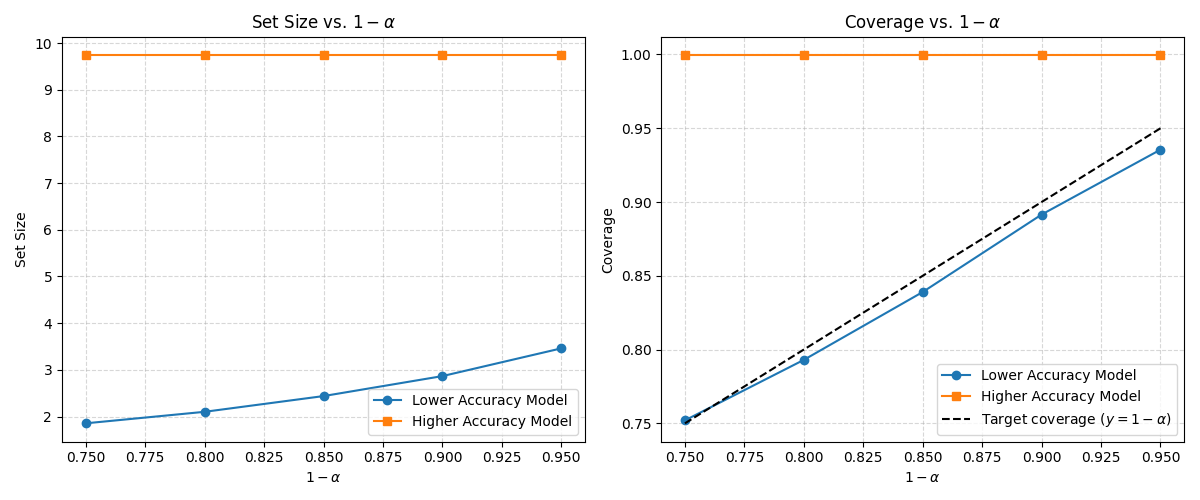
\includegraphics[width=\textwidth]{graphs/conformal_adaptive_comparison.png}
        \caption{Same as the above Figure \ref{fig:simpleCP-comparison}, but now using the APS strategy as described above.}
    \label{fig:adaptiveCP-comparison}
\end{figure}

Despite the APS approach being theoretically better, the results in Figure~\ref{fig:adaptiveCP-comparison} 
are not what we expect. The issue here is that with the higher accuracy model, 
the model generates one softmax score as essentially $1$, and the others at essentially $0$. 
As a result, there are many ties among the scores: the partial sums are all essentially $1$, 
leading to the unintendended behavior of including all $10$ categories in the prediction sets. 
The standard way to deal with tied scores is to introduce a random noise component in the scores, which we do in Figure~\ref{fig:RandomAPS-comparison}.

\begin{figure}[h]
    \centering
        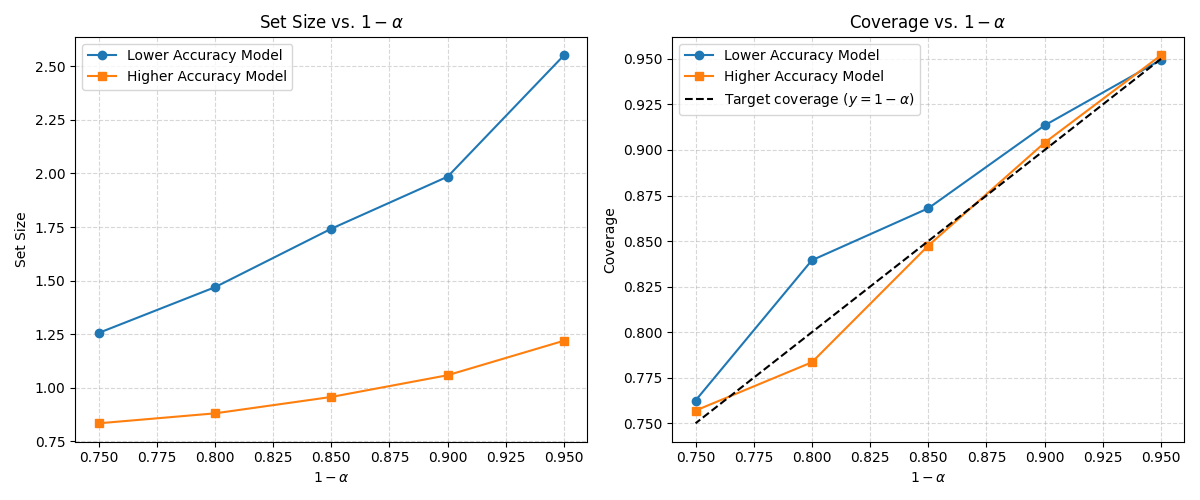
\includegraphics[width=\textwidth]{graphs/conformal_adaptive_random_comparison.png}
        \caption{Same as the above Figure \ref{fig:adaptiveCP-comparison}, but now using the randomized noise added to the scores as described above.}
    \label{fig:RandomAPS-comparison}
\end{figure}

A variation on the randomized version of APS is the regularized APS algorithm, which aims to both break ties using random noise, but also disincentivize large sets using a \emph{regularization} component, which discourages it from producing too large prediction sets. This algorithm is described in more detail in \cite{rapspaper}. Let $o_x(y)$ be the rank of $y$ in the output probabilities. 
    Moreover, we'll use two parameters $\lambda$, $k$ to determine how much we regularize the sets. Then,
    \[ s(x, y) = \max(0, \lambda(o_x(y) - k)) + p(y) \cdot u + \sum_{p(y') > p(y)} p(y'), \]
    where $u$ is random in $(0, 1)$. Thus, if for example $k=4$, including anything past the $4$th term
    now carries an extra penalty of $\lambda$, which means we are incentivized to use sets that don't include anything past the $4$th term, hopefully making the set sizes smaller.
    The results of this are in Figure~\ref{fig:regularizedCP-comparison}. 

\begin{figure}[h]
    \centering
        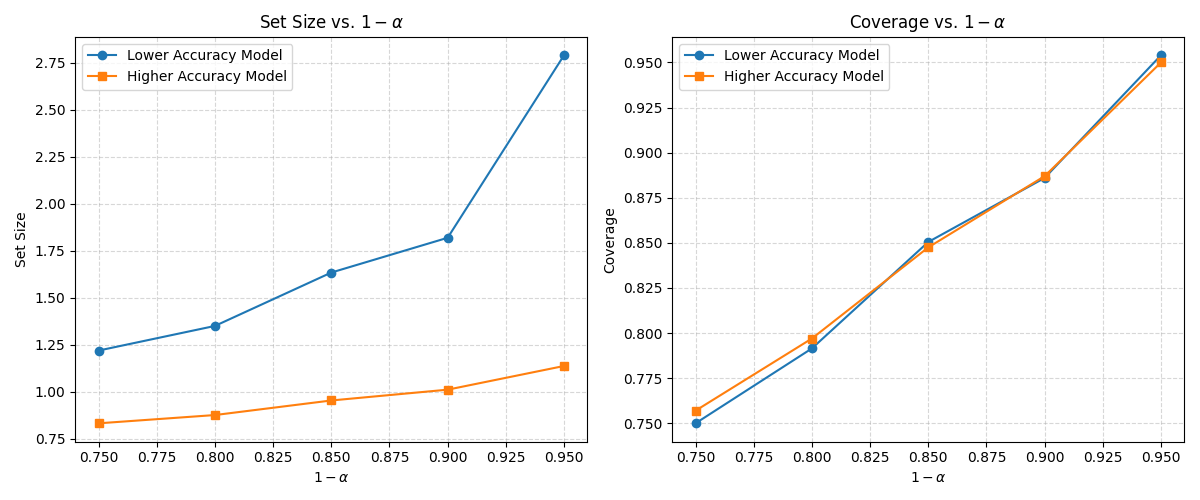
\includegraphics[width=\textwidth]{graphs/conformal_regularized_comparison.png}
        \caption{Using the regularized RAPS algorithm on MNIST, with $k = 3$, $\lambda = 0.1$.}
    \label{fig:regularizedCP-comparison}
\end{figure}

In our case, for an MNIST classifier, the impact of using RAPS versus a simple random noise based strategy is not too large. 
With only ten labels, everything past the first few labels has probability of essentially zero, and would not be included anyway. H
owever, RAPS can make a bigger difference on classification tasks like ImageNet.
When we have large class spaces $Y$ like in ImageNet, then a tail of small probabilities forms, and RAPS stops us from including classes from the tail.

\section{Regression}
\label{sec:regression}
Another use case for conformal prediction is when we have a regression model instead of a classification model.
For a simple version of CP for regression, we will start with a \emph{quantile regression} model. Given some data $x$, 
it will give us a prediction \emph{interval} $(t_{\alpha/2}, t_{1 - \alpha/2})$ that should contain the correct value $y$ 
with coverage of $1 - \alpha$. But in order to statistically guarantee $1 - \alpha$ coverage, we can apply conformal prediction. 
Define the score of $(x, y)$ to be how far $y$ is from the predicted quantiles, that is, 
\[ s(x, y) = \max(t_{\alpha/2} - y, y - t_{1 - \alpha/2} ) .\]
Because of the way we have defined this score function, if $y$ indeed lies within the predicted interval, 
the score $s(x, y)$ will be negative, and it will be positive if $y$ is outside the interval. Our analogue of 
including elements in the prediction set will then be to widen the interval based on $\alpha$, so the conformalized
interval is $(t_{\alpha/2} - \hat{q}, t_{1 - \alpha/2} + \hat{q})$. The results of using this algorithm, known as \emph{CQR}
are shown in Figure~\ref{fig:simpleRegression-comparison}.

\begin{figure}[h!]
    \centering
    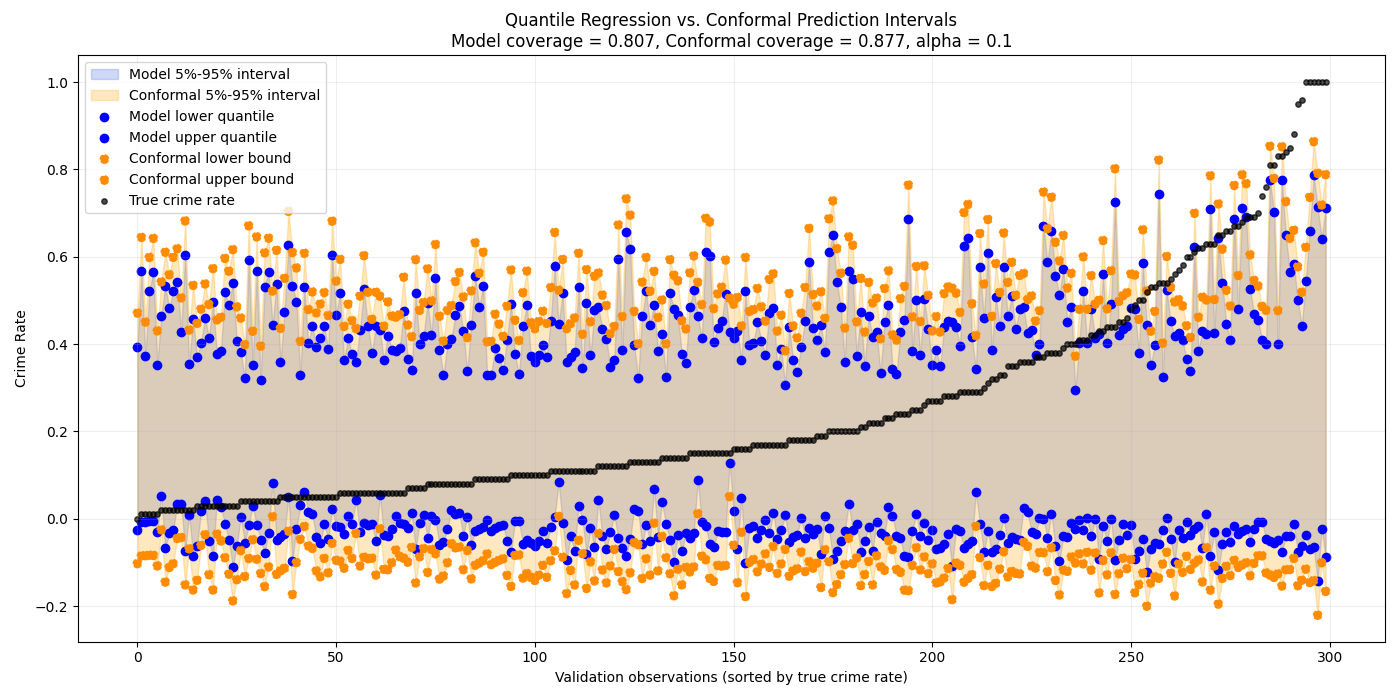
\includegraphics[scale=0.4]{graphs/badNNregressionCQRscatterV2.png}
    \caption{CQR on the \emph{Crimes and Communities Dataset}, predicting the crime rate in a community based on data about communities. 
    Here $X$ contains sets of $122$ data points about communities, and $Y$ is the crime rate.}
    \label{fig:simpleRegression-comparison}
\end{figure}

As an alternative to the CQR algorithm, we can adjust the prediction sets in a more adaptive way, 
depending on both $\hat{q}$ as well as some estimate of the uncertainty of a prediction. In this case, 
we begin with a model that estimate $y$ from $x$, producing $\hat{y}$. We then use a second model to predict
some uncertainty scalar $u(x)$: this can be an estimate of the residual, standard deviation, or something else.
The scores are then 
\[ s(x, y) = \frac{| \hat{y} - y |}{u(x)} , \]
and the prediction sets are constructed as $(\hat{y} - \hat{q}u(x), \hat{y} + \hat{q}u(x))$.
This method, called \emph{Uncertainty Scalars} is shown in Figure~\ref{fig:UncertaintyScalars}.

\begin{figure}[h]
    \centering
    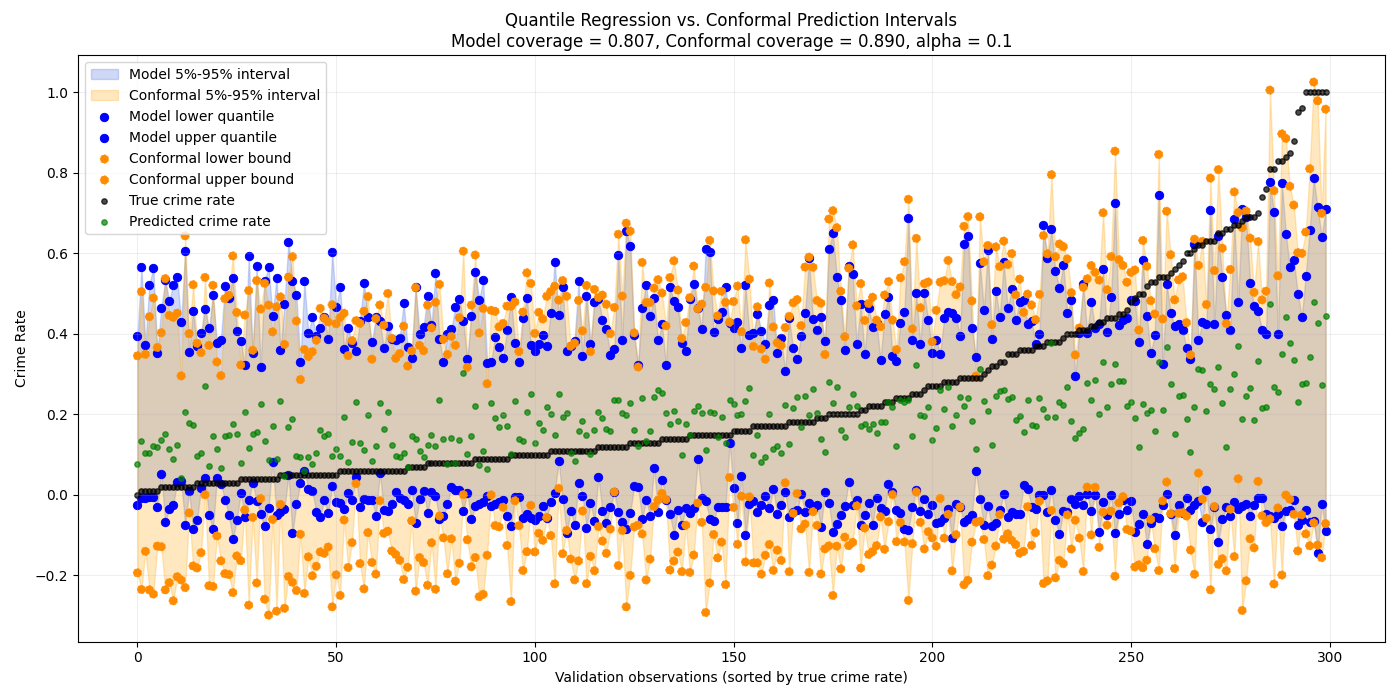
\includegraphics[scale=0.4]{graphs/NNregressionAdaptive_badV2.png}
    \caption{Uncertainty scalars given by $u(x) = |t_{1 - \alpha/2} - t_{\alpha/2}|$ with a model predicting both the true value as well as the quantiles on Crimes and Communities.}
    \label{fig:UncertaintyScalars}
\end{figure}

\section{Text}
\label{sec:text}
Trying to apply conformal prediction techniques to the case of a language model generating answer to questions
poses a more difficult challenge. For one, text outputs are much less structured than a classification or regression scenario.
For instance, multiple different-looking outputs can really be the same answer. Moreover, there is effectively an infinite space of possible outputs.
Also, we (in general) will not have any more information from a query $x$ than what the model will output, since we are dealing
with black-box models and know nothing about assigned probabilities. Given these hurdles, how can we assign scores $(x, y)$?
It's clear that we will need to sample the model many times in order to get any information. Then the simplest thing 
that we can do here is to compute probabilities from these $n$ outputs:
\[ p(y) = \frac{\text{\# of times $y$ was outputted}}{n}, \]
and let $s(x, y) = 1 - p(y)$. Immediately, we run into an issue: many equivalent outptuts $y_i$ can be slightly different, 
and so counted as different by this probability even though they are really not. Thus, we must perform \emph{semantic clustering} on the results. That is, we group the results $y_1, \dots, y_n$ into clusters $Y_1, \dots, Y_k$ containing
equivalent responses. One way to do this is to simply ask the model itself to judge entailment between two responses; 
then $y_i \equiv y_j$ when $y_i$ entails $y_j$ and $y_j$ entails $y_i$. \medskip

To test these algorithms, we evaluate on a subset of the TriviaQA dataset, which contains one-line trivia questions 
and answers, using Qwen3-8B to answer questions, as well as to judge entailment. It is worth noting that the Qwen3-8B model
is not very accurate on this dataset by itself: it only achieves around $50\%$ accuracy on a single response. We run the above algorithm, with a range of $\alpha$s and $15$ queries per question in Figure~\ref{fig:simpleCPQ}. \medskip

However, as seen in Figure~\ref{fig:simpleCPQ}, the coverage plateaus around $0.55$, and so we do not meet the conformal 
coverage guarantees. The problem here is that with the $n$ queries we make to the model, it's possible the true $y$
was simply not in any of the clusters produced. If this happens with probability more than $1 - \alpha$, there is nothing we can do to save face. If the answer is not produced in the $n$ queries, no subset will ever contain the answer. 


%%\begin{figure}[h]
 %%       \centering
  %%      \includegraphics[width=0.5\textwidth]{FreqHighMin1malpha_vs_coverage.png}
    %%    \vspace{1cm}
      %%  \includegraphics[width=0.5\textwidth]{FreqHighMin1malpha_vs_setsize.png}
        %%\caption{Coverage and Set Size vs $1 - \alpha$ for the algorithm described above. As we can see in the graph, the coverage plateaus, and we cannot guarantee coverage.}
        
        %%\label{Coverage-SimpleCPQ}
        
%%\end{figure}
\begin{figure}[ht]
\centering
\resizebox{\textwidth}{!}{%
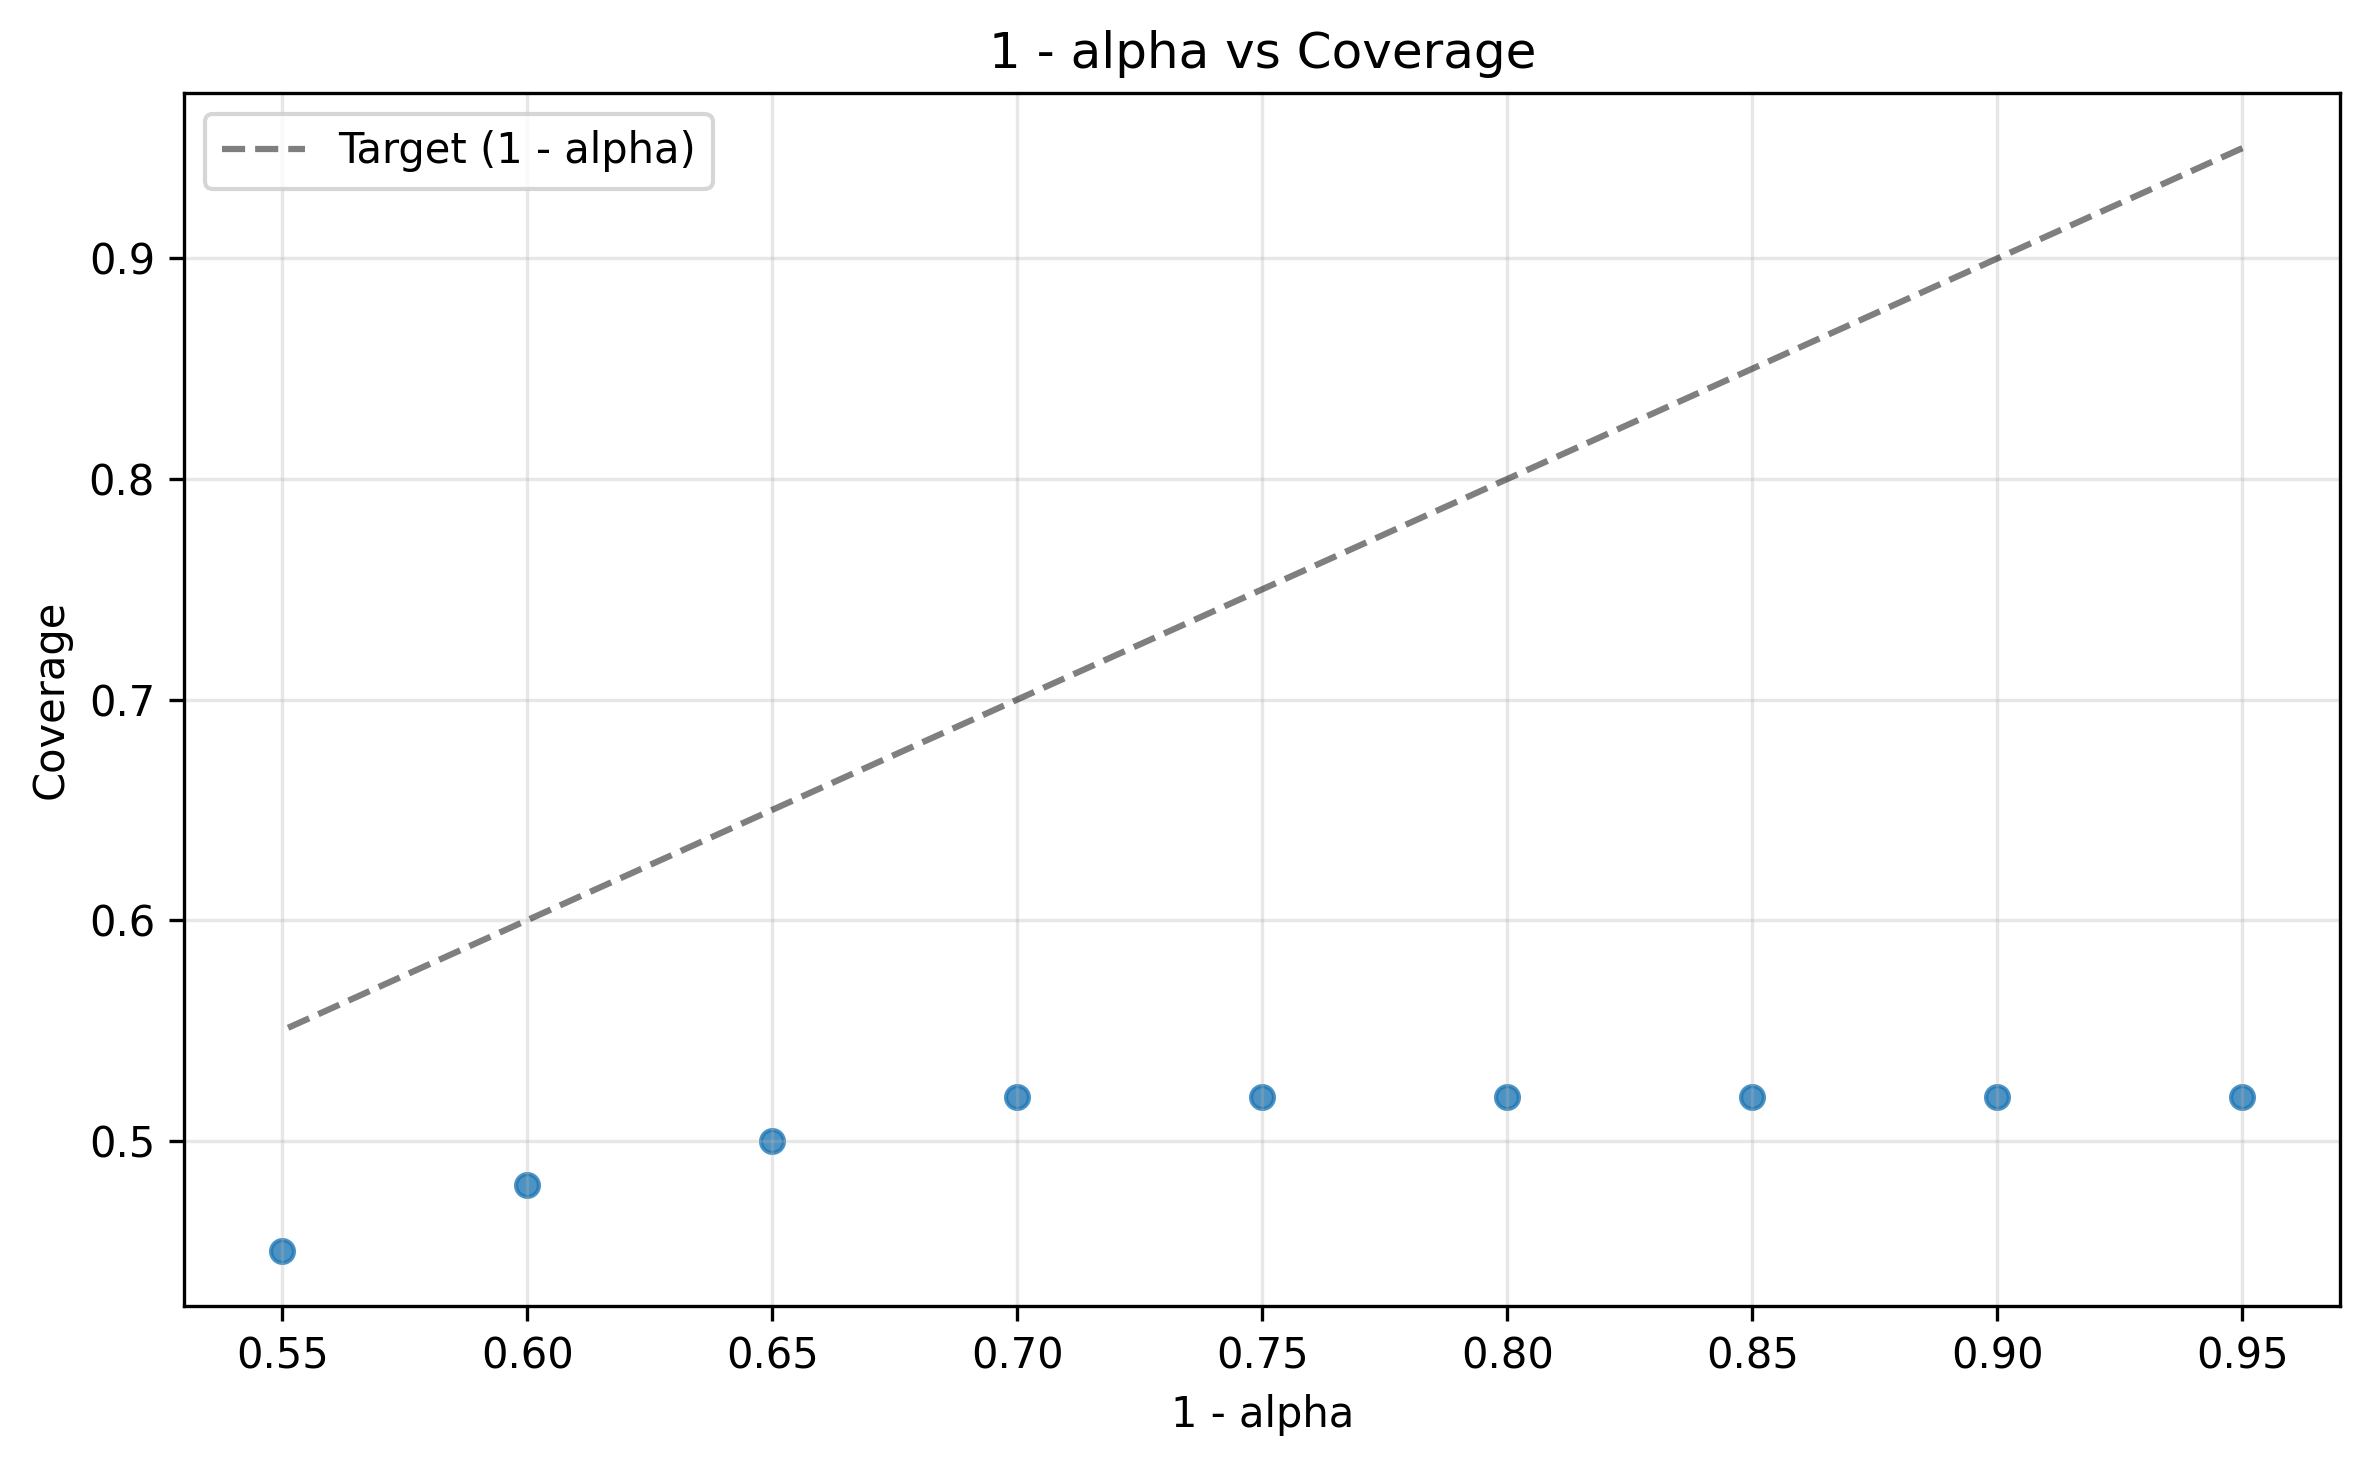
\includegraphics[height=5cm]{cpq/graphs/FreqHighMin1malpha_vs_coverage.png}%
\quad
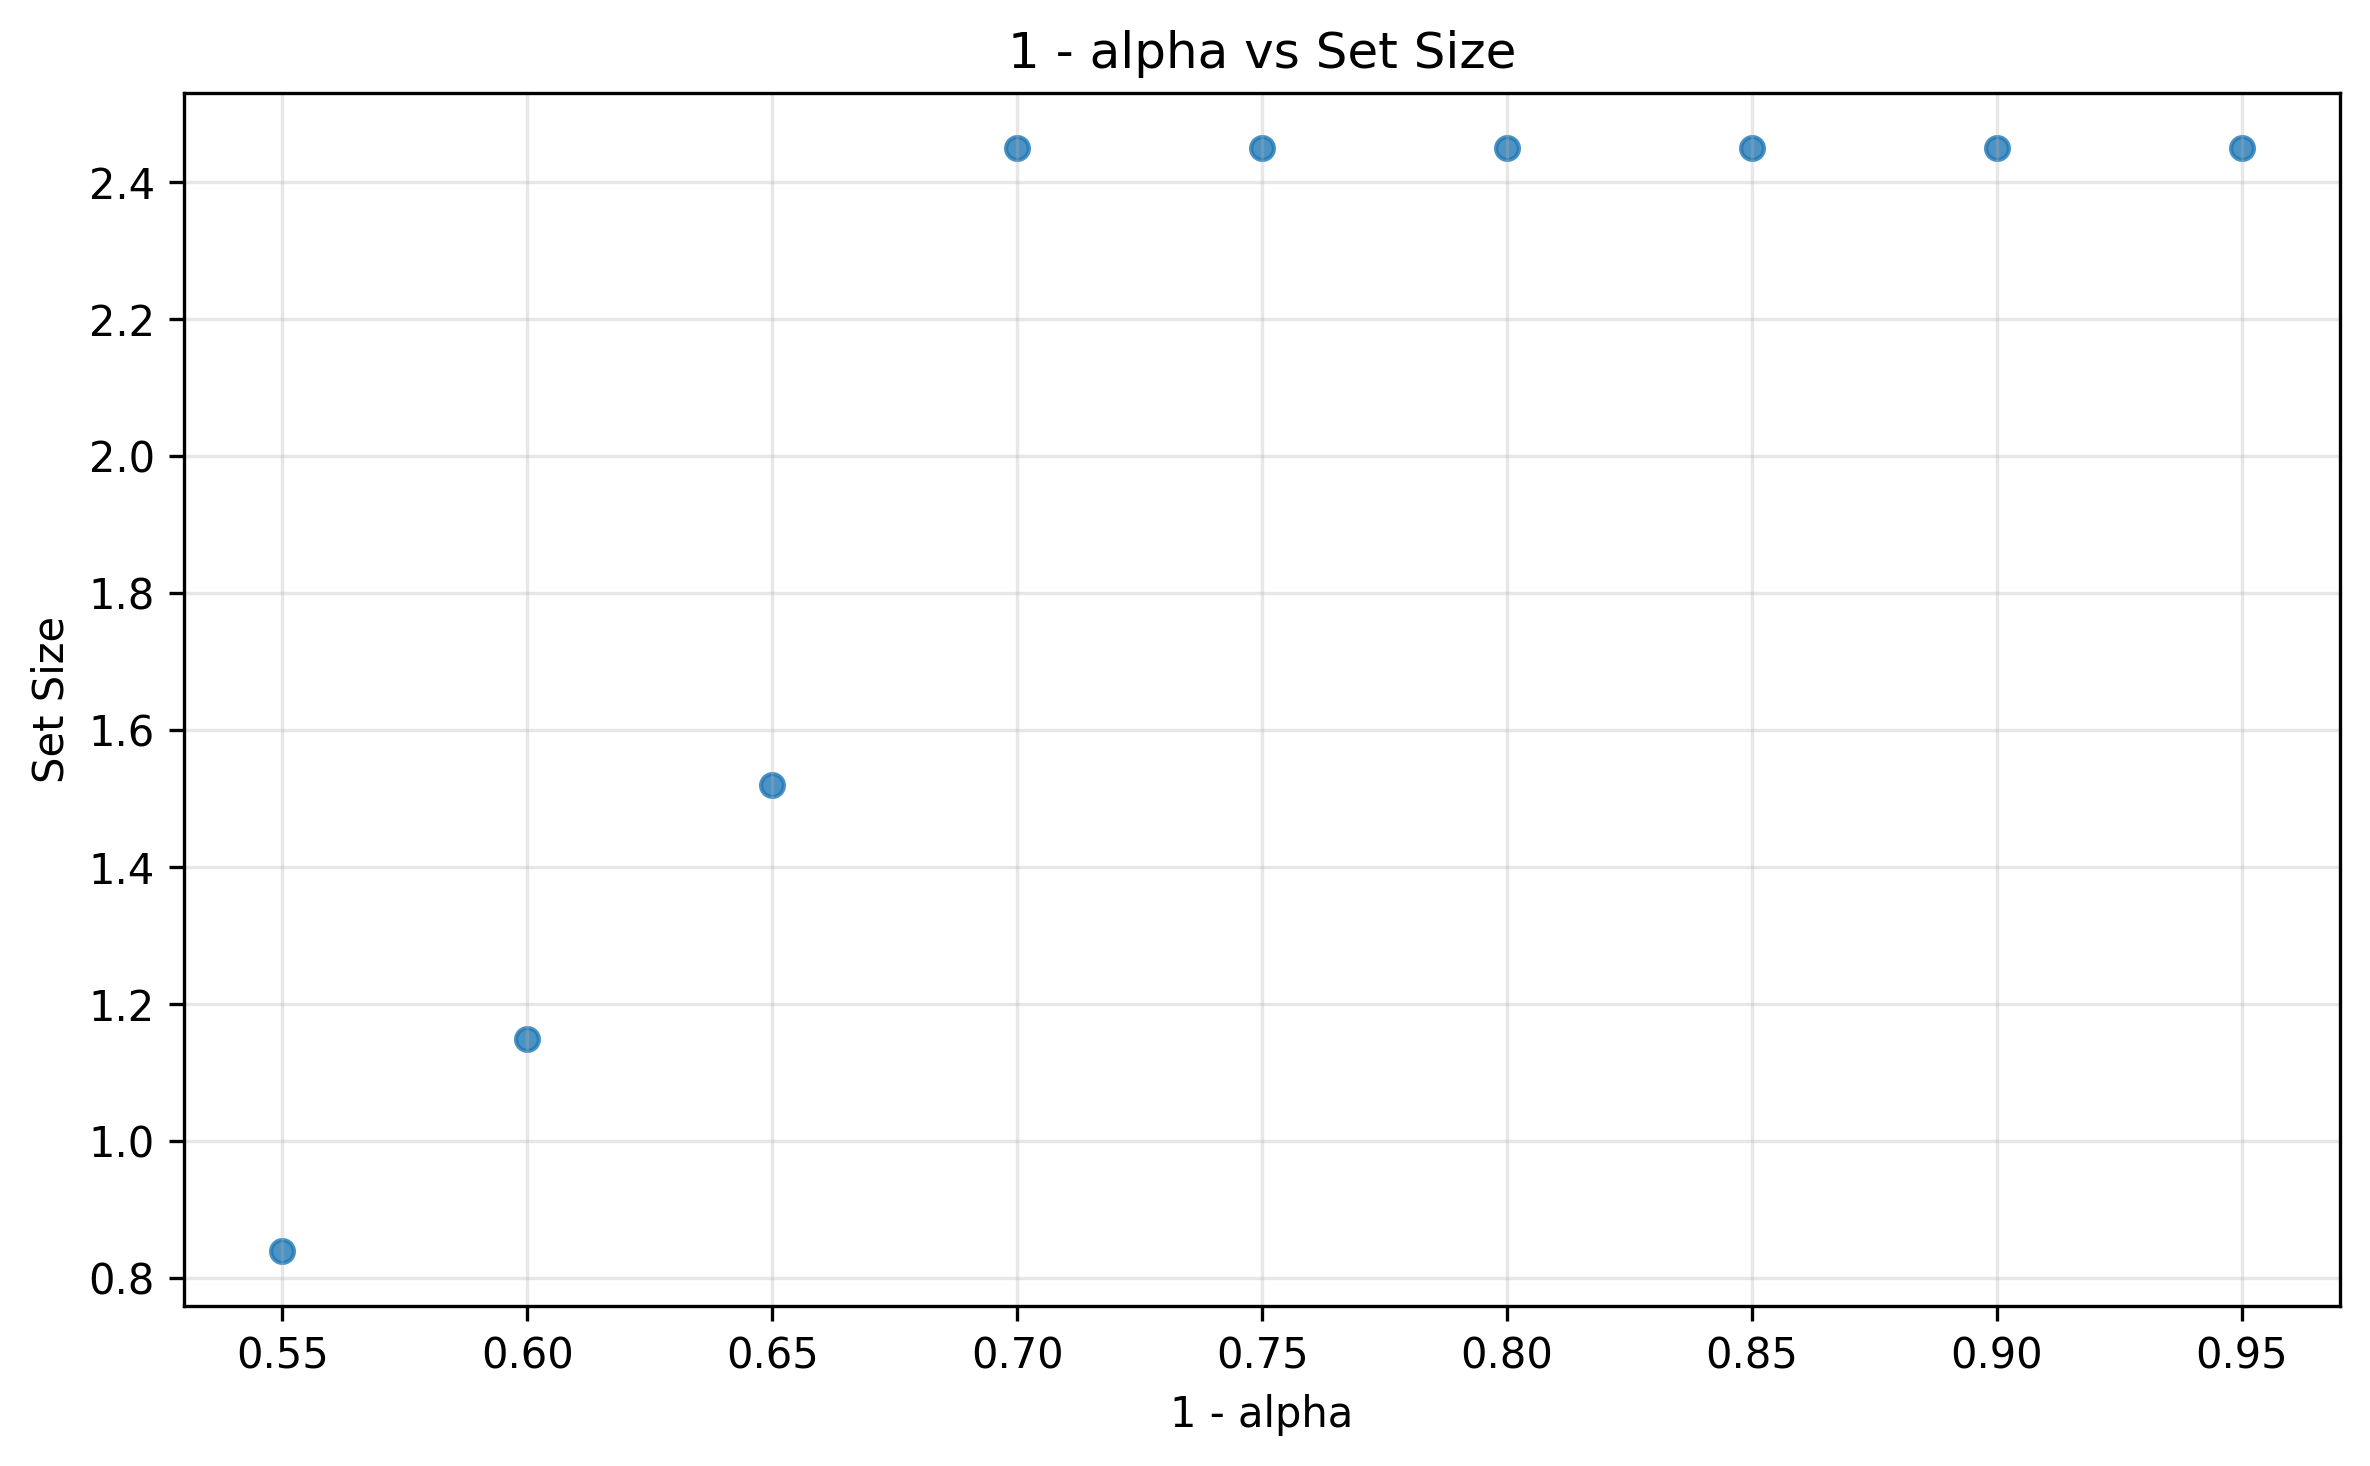
\includegraphics[height=5cm]{cpq/graphs/FreqHighMin1malpha_vs_setsize.png}%
}
\caption{Coverage and Set Size vs $1 - \alpha$ for the algorithm described above. 
  As we can see in the graph, the coverage plateaus, and we cannot guarantee coverage.}
\label{fig:simpleCPQ}
\end{figure}



In order to restore the guarantee of coverage, one option is to introduce an element $EE$(for \emph{everything else}) into the prediction set. If $EE$ is in the set, then we automatically have coverage. However, including $EE$ makes our sets much less informative by including an infinite number of options. Thus, we should try to discourage the presence of $EE$ by making the scores $s(x, EE)$ higher than the scores for actual answers $s(x, y)$. Our estimate for the probability of $EE$ should be the probability that the answer is \emph{not} any of the answers already seen. This is the missing probability mass of the clusters. Given this quantity $\theta(x, t)$, computed from $t$ examples, we define the score
\[ s(x, EE) = 2 - \theta(x, t) , \]
and the score of $y \neq EE$ as 
\[ s(x, y) = 1 - \omega(y \mid  x) , \]
where $\omega(y | x)$ is the probability of $y$ given the sequence of $t$ samples. 
Using the two minus term in the $s(x, EE)$ scores effectively disincentivizes the model from including $EE$, since the scores $s(x, EE) \in (1, 2)$ are strictly greater than any scores $s(x, y) \in (0, 1)$.
But how can we measure the missing mass? The \emph{Good-Turing} estimator for missing mass is 
\[ \hat{\theta}(x, t) = \frac{N_1}{t} = \frac{\text{\# number of clusters that appear exactly $1$ time}}{t} , \]
which is what we use to comopute the scores for $s(x, EE)$. For the scores of other $y$, we could simply use the frequency based estimators as earlier, but a more robust strategy is to use a turing estimator for this as well. If $y$ is seen $r$ times in our $t$ samples, set
\[ \hat{\omega}(y \mid x)  = \frac{r + 1}{t} \frac{N_{r + 1}}{N_r} , \]
where $N_r$ denotes the number of clusters seen exactly $r$ times. The reason that this is better is that Turing Estimators include the possibility that the answer is not in the set, i.e these probabilities will not necessarily sum to $1$, so there is some missing mass which is accounted for by the estimators. \medskip

To use this algorithm, one more component is needed. The \emph{query policy} determines the number of times we will sample the model. Naturally, sampling more is better, but querying the model is expensive and we cannot do it as many times as we please. The aim is to use a policy that is adaptive to the question, but ensures that the average number of queries will be $\le$ the user-set query budget $B$. The way that we will make our query policy adaptive is to, essentially, query until the point of diminishing returns. To quantify this, we again look toward the missing mass. Our policy will be to query until 
\[ \theta(x, t + 1) - \theta(x, t) > \beta^* ,\]
where $\beta^*$ is some negative threshold value. We prove that this is an optimal query policy in Claim~\ref{querypolicy}. Effectively, we are the change in $\theta(x, t)$ as a measure for how much information 
the query has given us. If the missing mass decreases by only a little, then the query is not very informative, and we have reached the point of diminishing returns. As far as computing this quantity, we (again) use a Good-Turing estimator. Let 
$\Delta(x, t) = \theta(x, t + 1) - \theta(x, t)$. Then our estimator for the change in missing mass is 
\[ \hat{\Delta}(x, t) = \frac{N_2}{t^2} . \]
We also have to choose a value of $\beta^*$ that will maintain our query budget $B$. To do so, we run the query policy over a range of $\beta$ values, and choose the largest value that still has average number of queries $\le B$. This full algorithm is known as \emph{CPQ}, introduced in \cite{cpqpaper}.


\begin{figure}[ht]
\centering
\resizebox{\textwidth}{!}{%
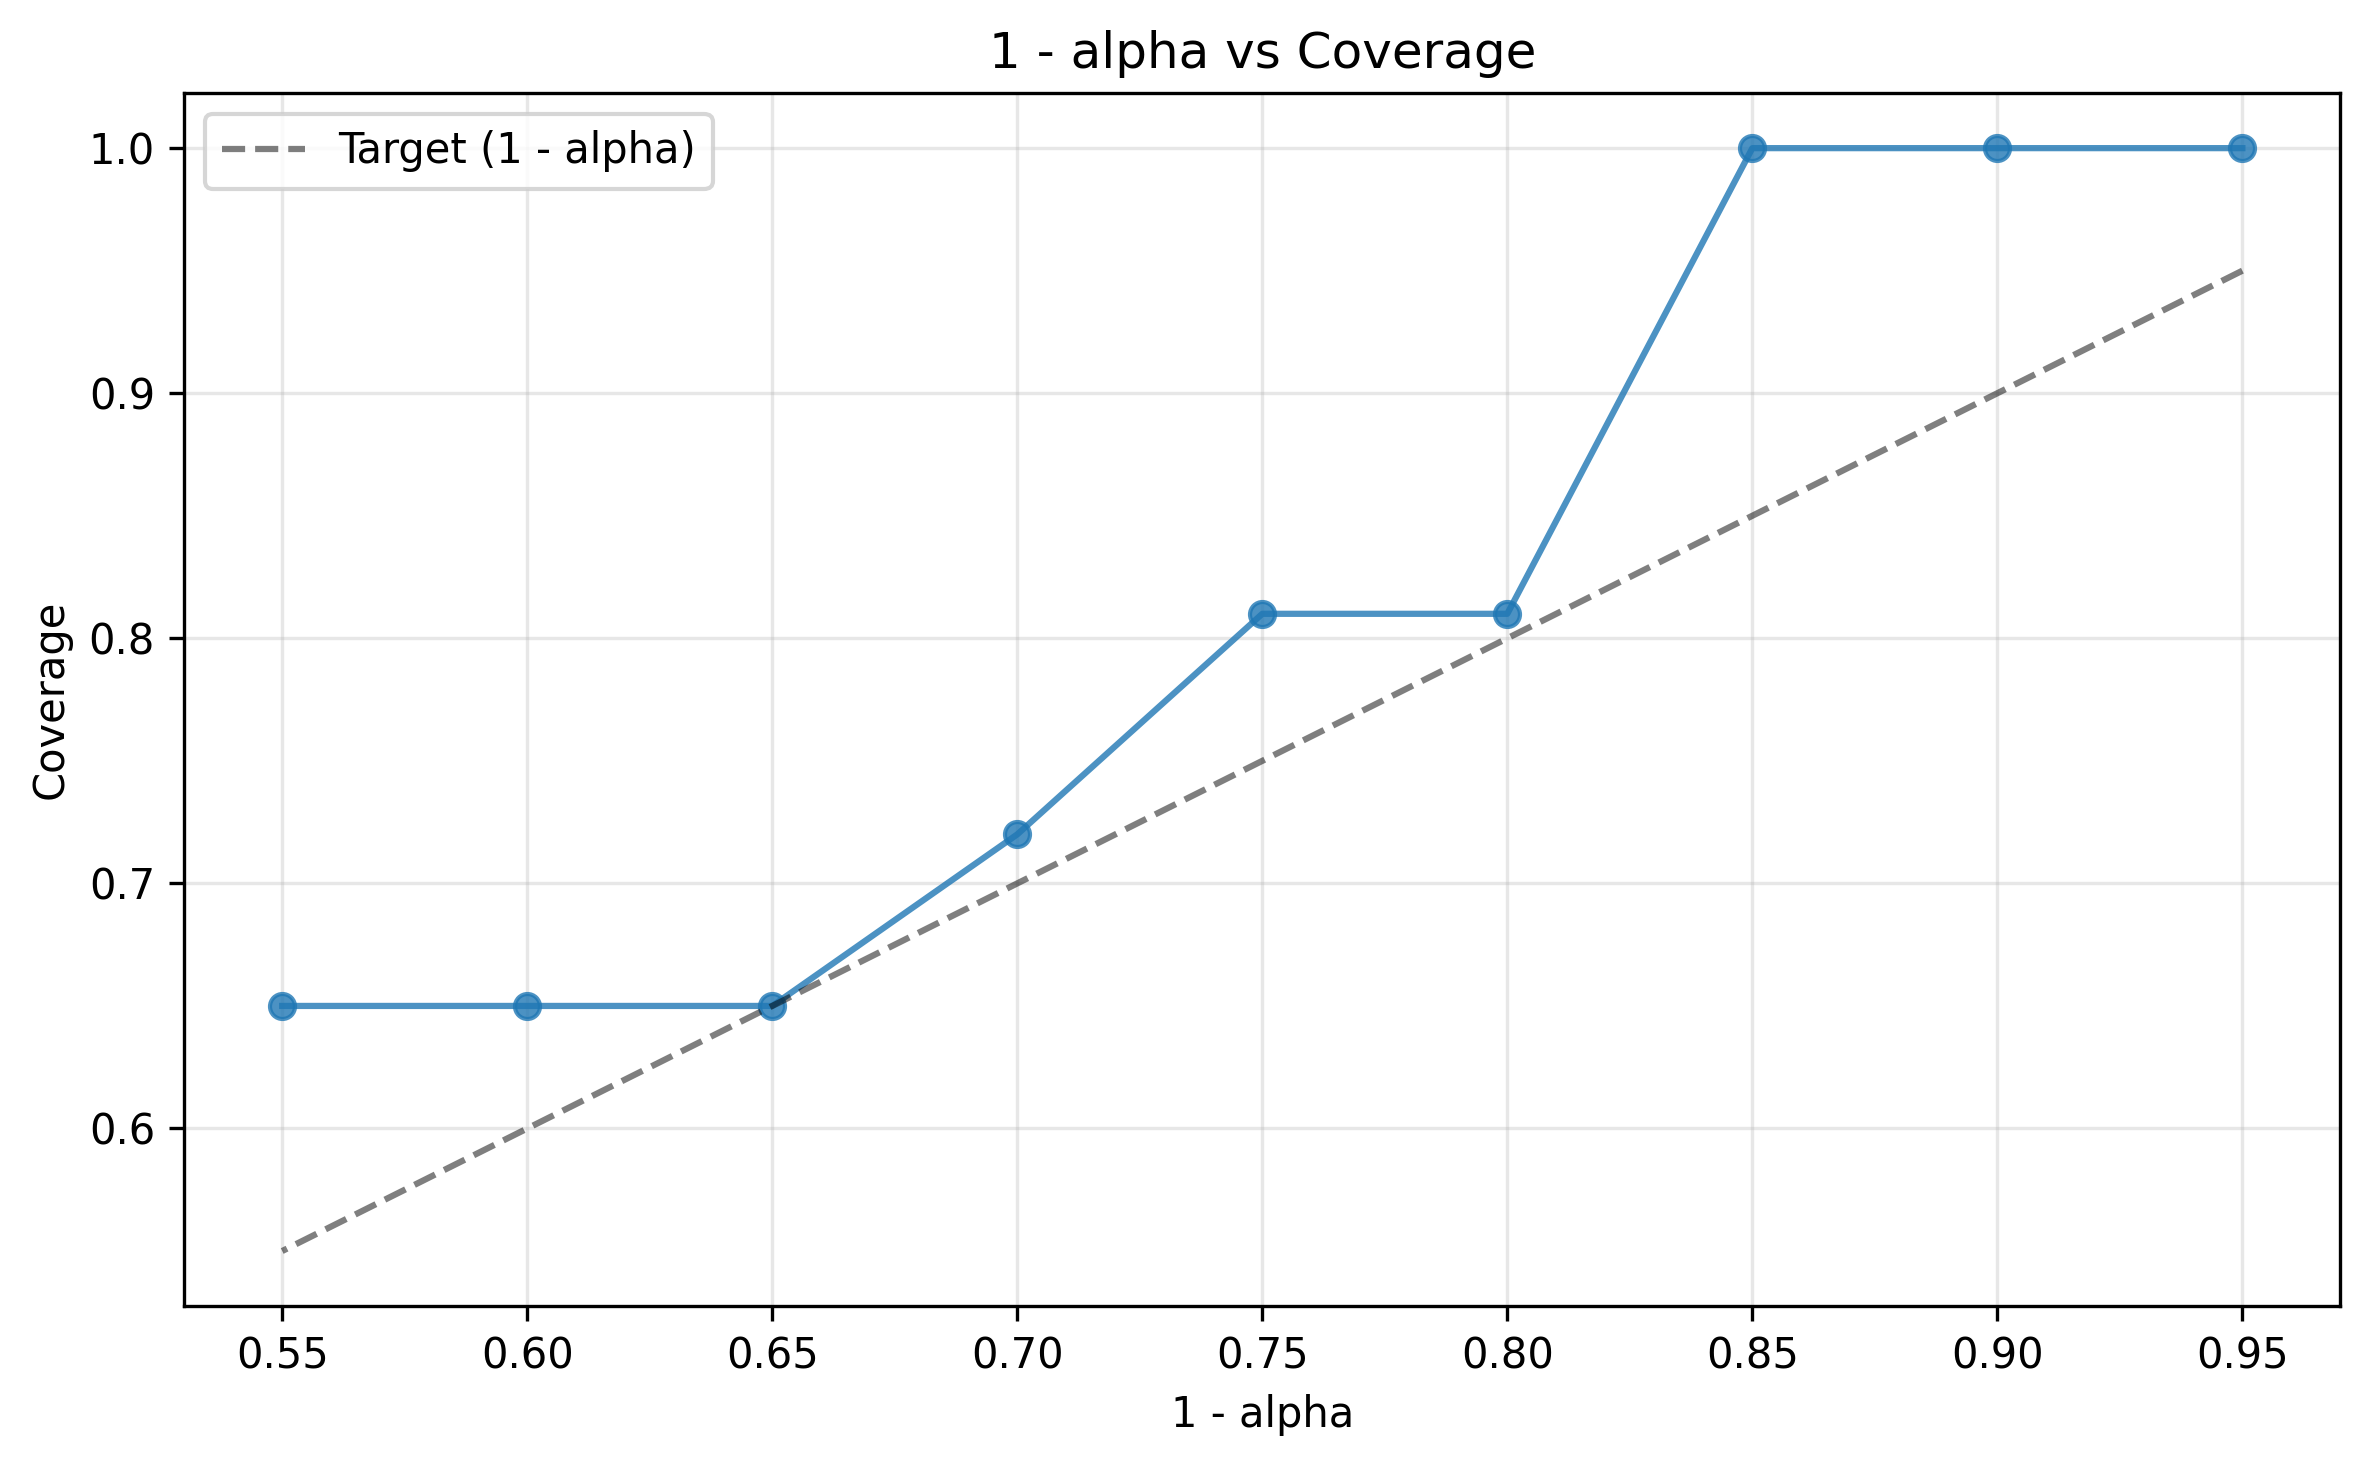
\includegraphics[height=5cm]{cpq/graphs/HighMin1malpha_EE_vs_coverageV1.png}%
\quad
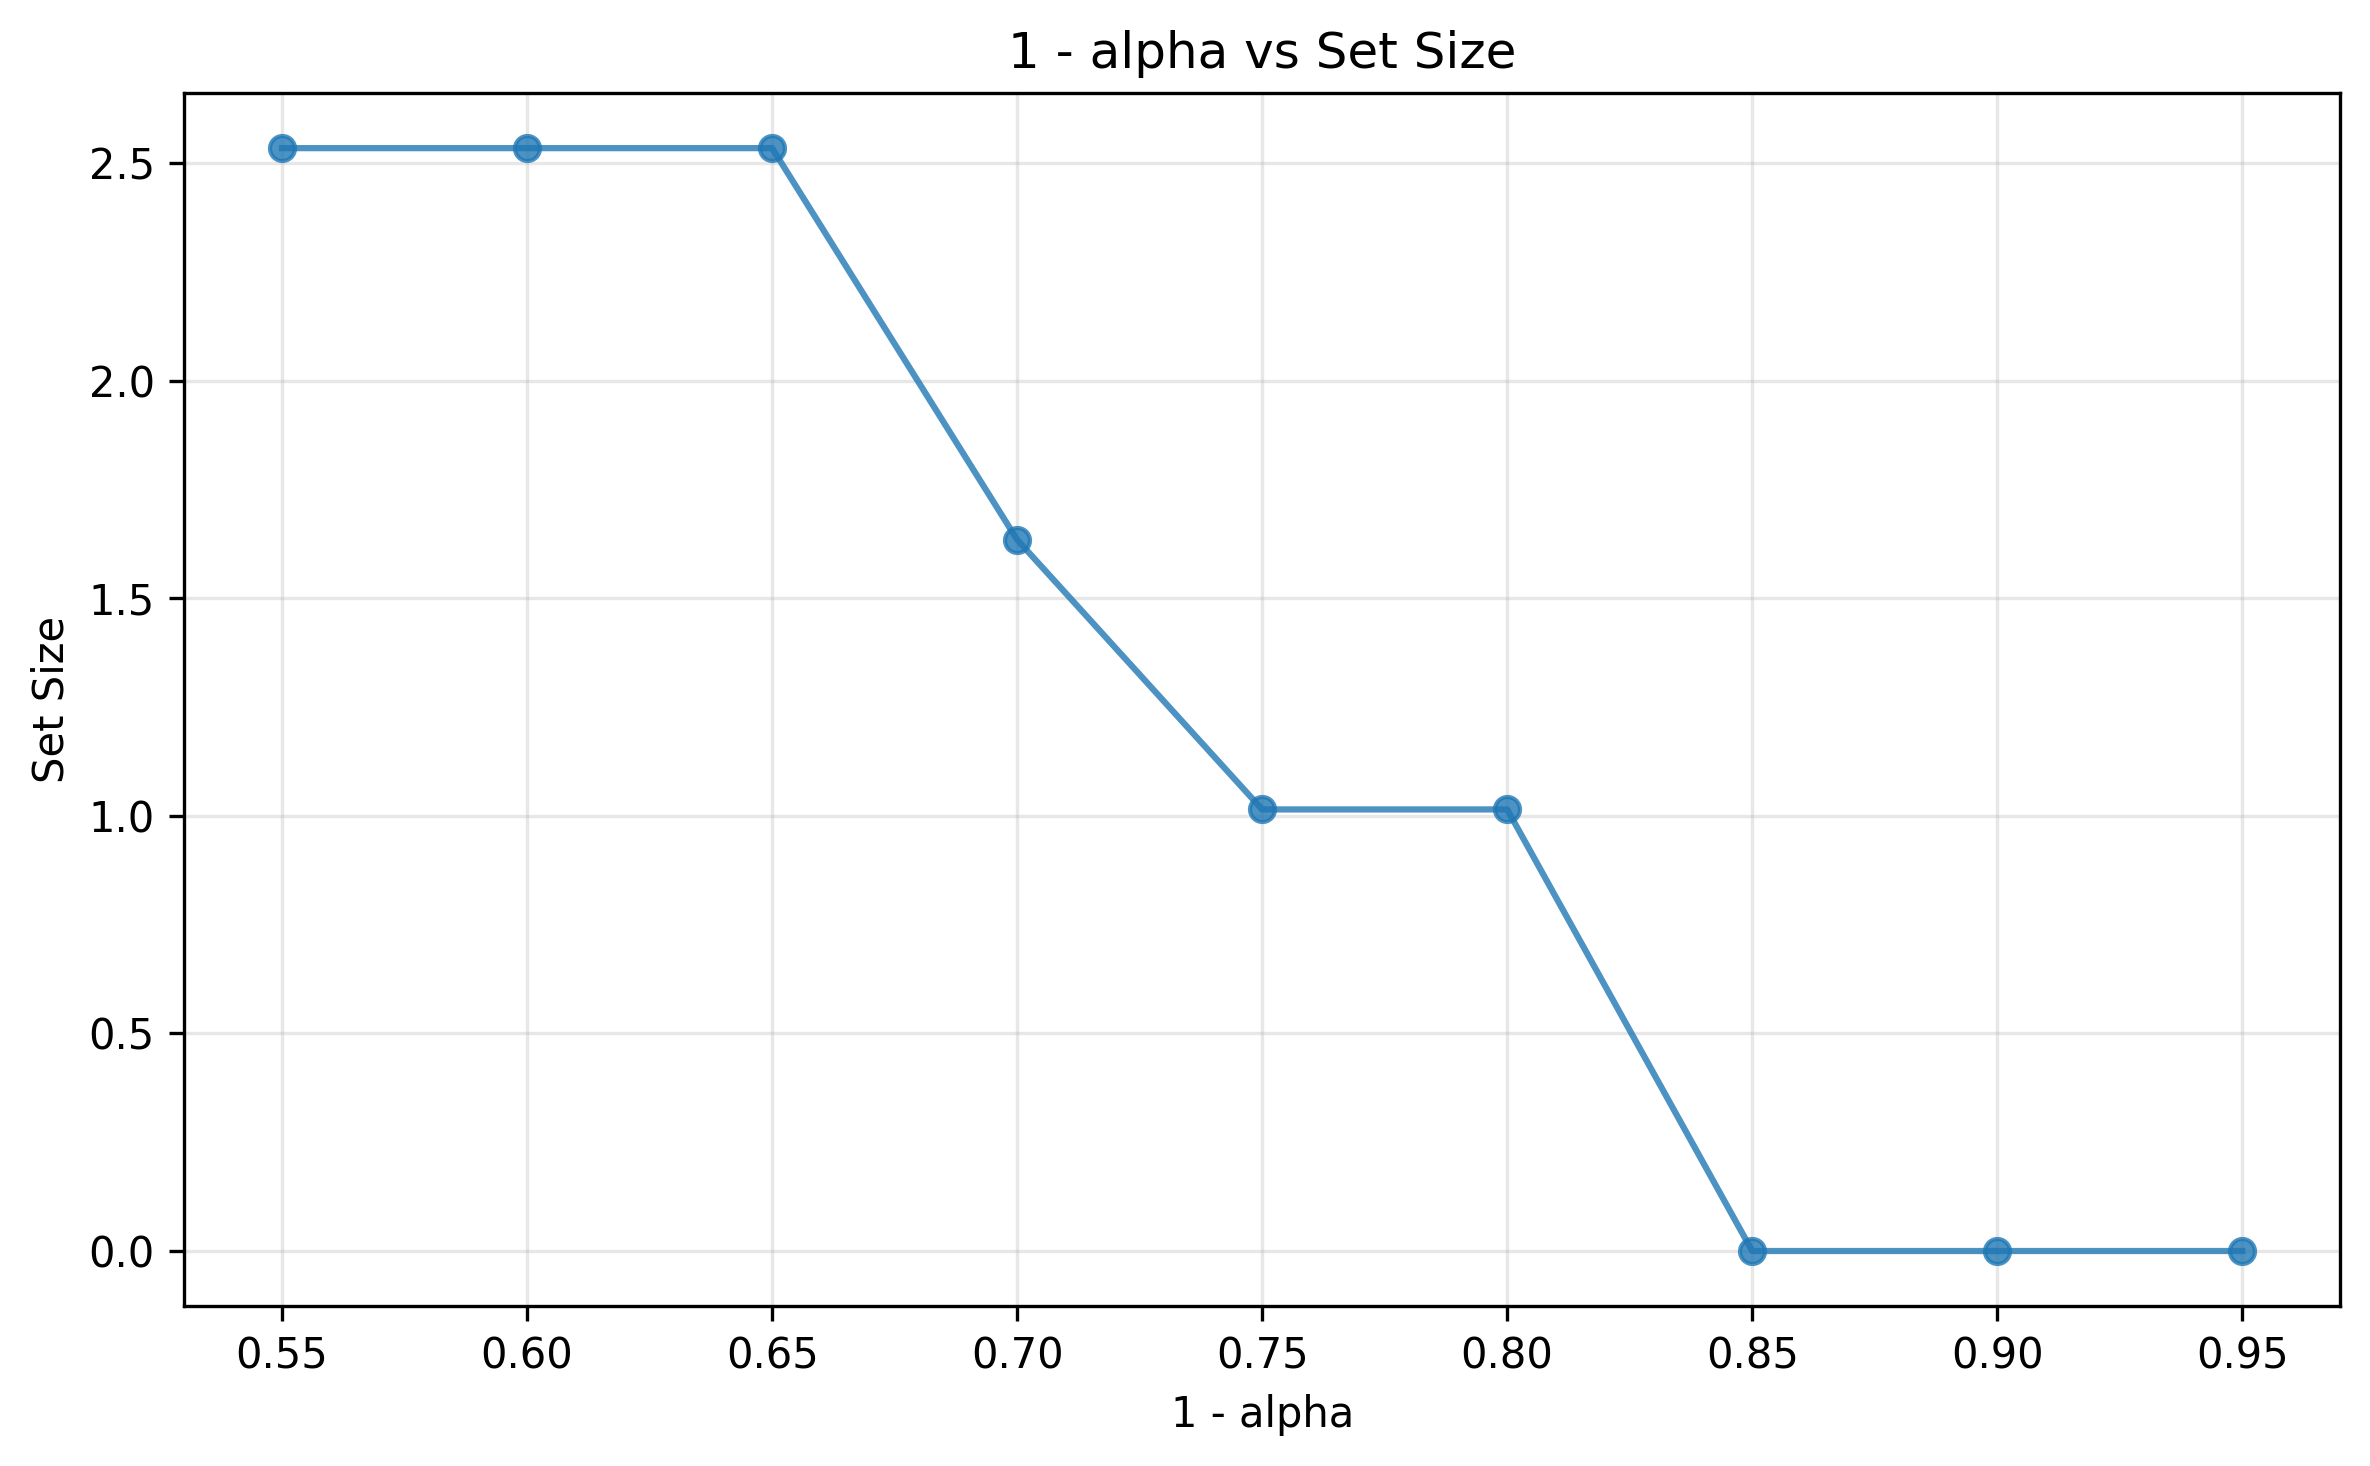
\includegraphics[height=5cm]{cpq/graphs/HighMin1malpha_EE_vs_setsizeV1.png}%
}
\caption{Coverage and Set Size vs $1-\alpha$ for the CPQ algorithm. The minimum number
of queries was $15$, and Qwen3-8B was the model used for entailment judging as
well as sampling answers on TriviaQA. Here, set size does not include EE.}
\label{fig:CPQ}
\end{figure}

For this CPQ algorithm, we can also plot the fraction of times $EE$ was included in the prediction set.
\begin{figure}[ht]
    \centering
    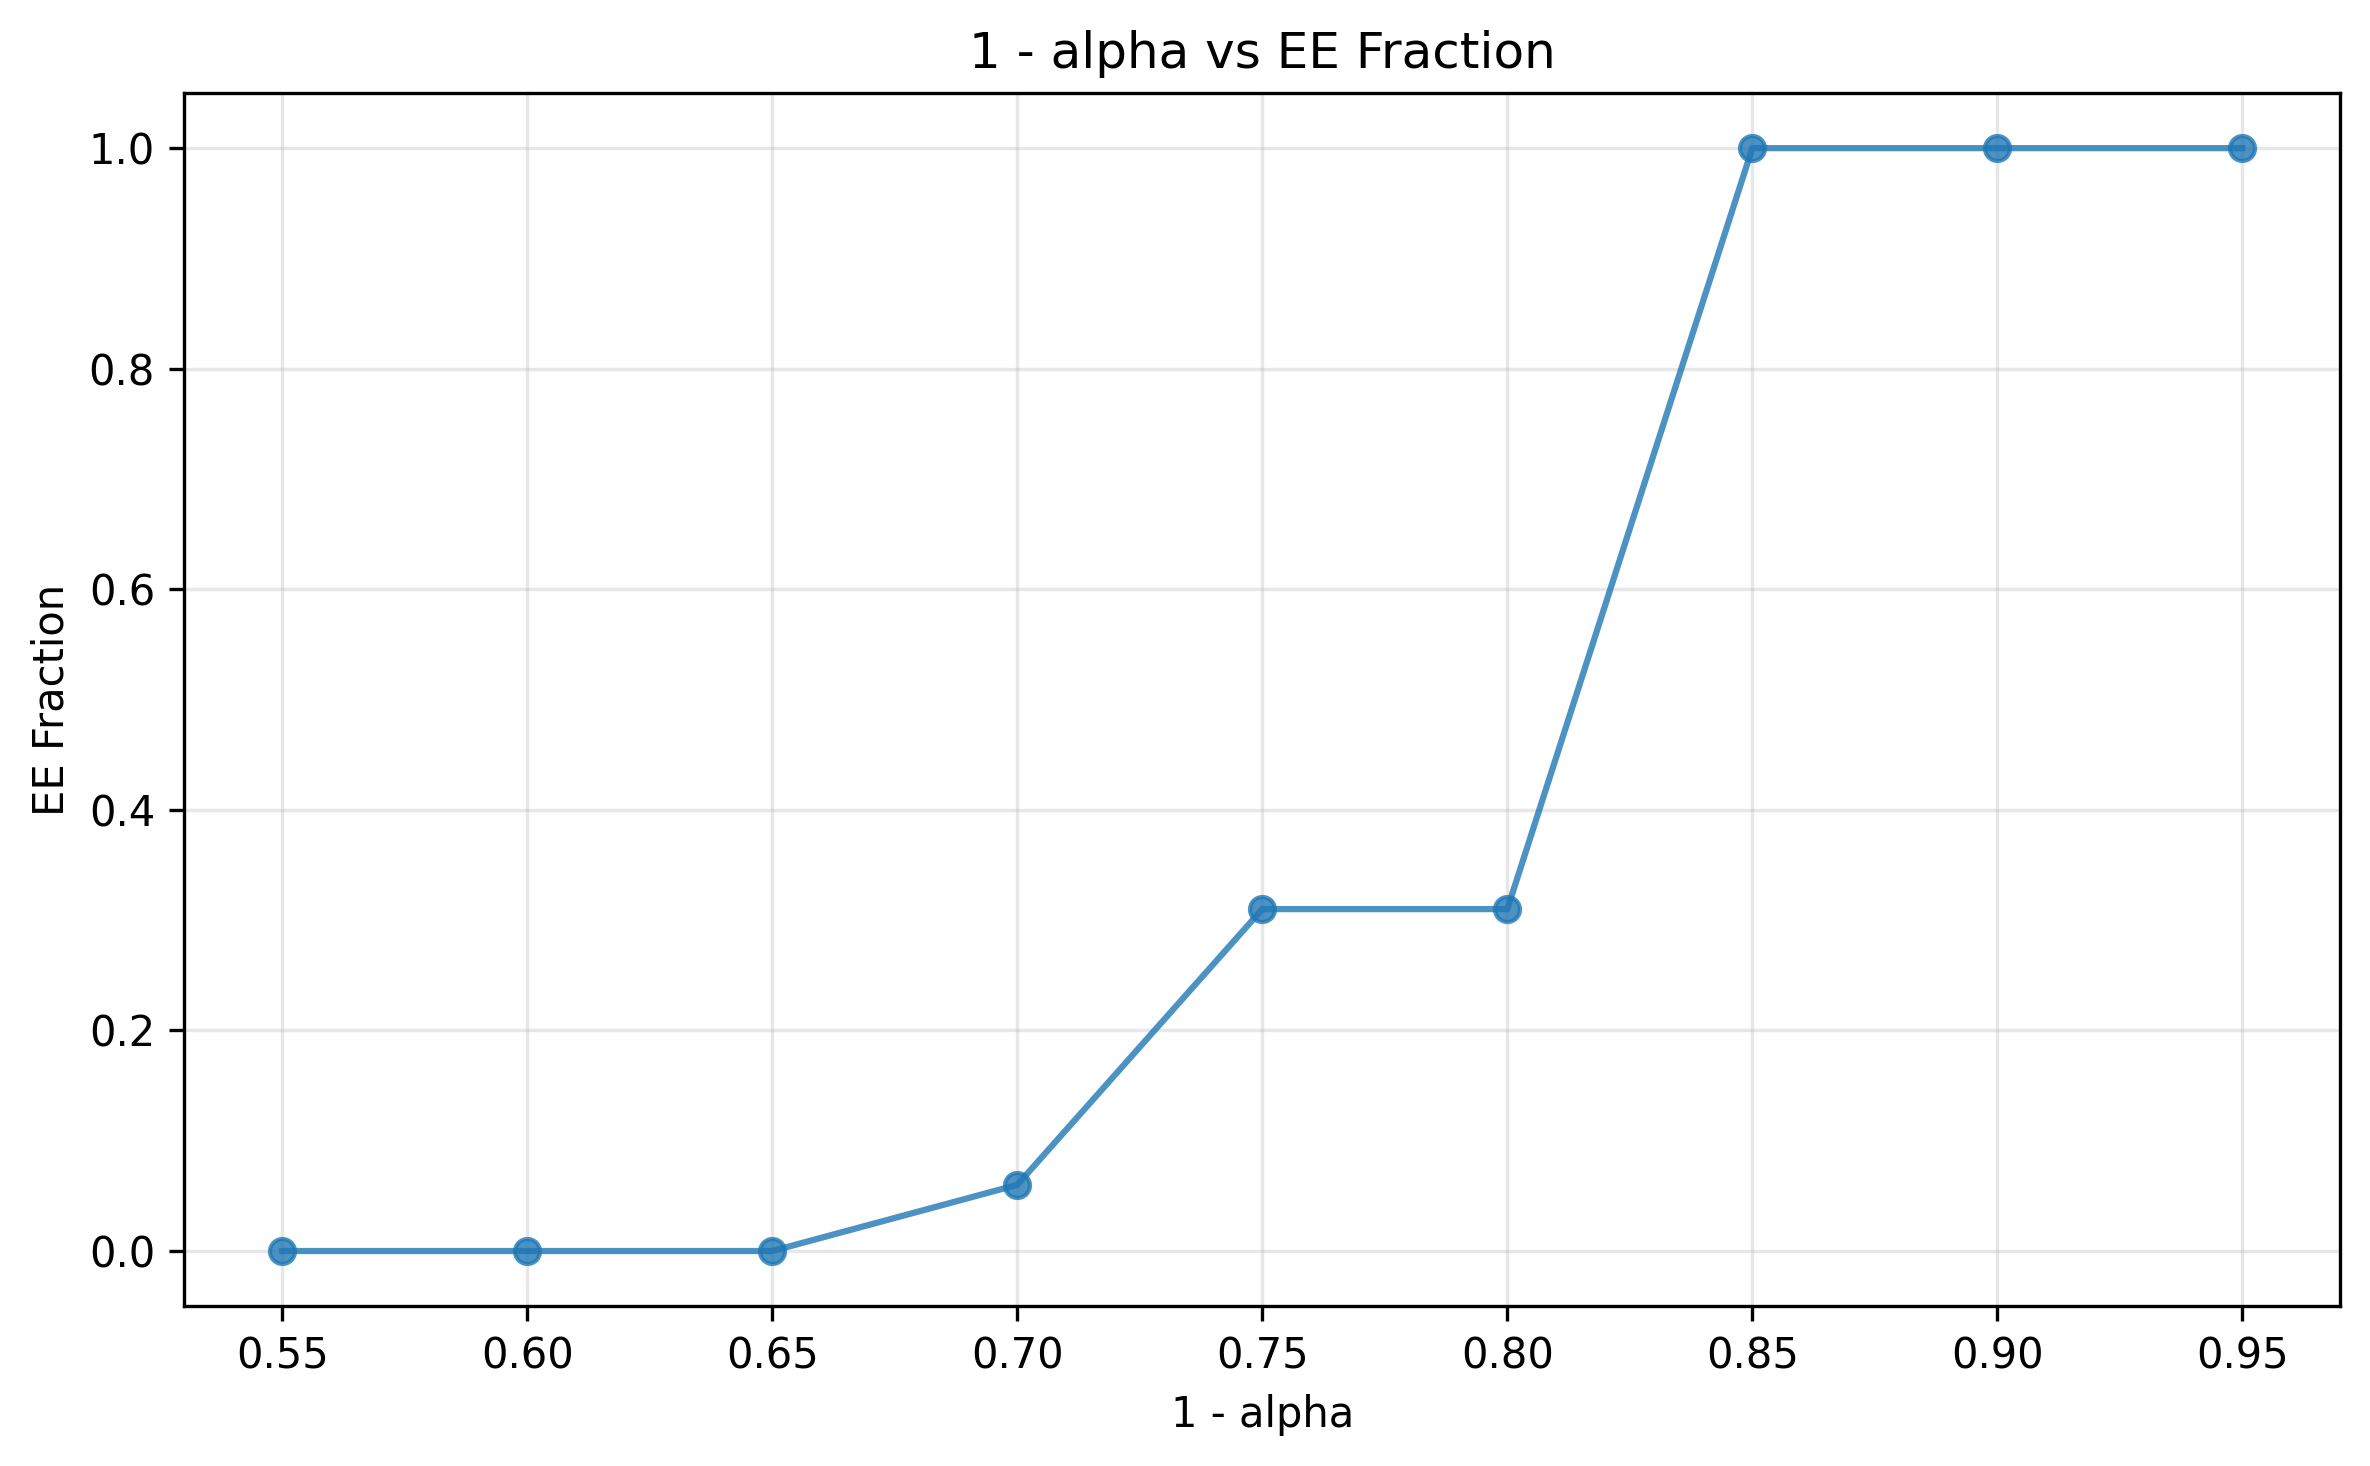
\includegraphics[scale=0.4]{cpq/graphs/HighMin1malpha_EE_vs_eefracV1.png}
    \caption{Fraction of times EE was included vs $1 - \alpha$ for the CPQ algorithm on TriviaQA as above.}
    \label{fig:CPQeefrac}
\end{figure}

As Figure~\ref{fig:CPQ} shows, including EE is finally able to guarantee coverage when the simple strategy could not. As the $EE$ fraction increases, the set size decreases because including more labels when EE is already included is redundant.
In our experiments, the values of $\hat{q}$ were always $\ge 1$ on the range of $\alpha$s tested. 
This means that every cluster produced by the model was included, 
so the only thing that changed with $\alpha$ was the fraction of the time we outputted $EE$. 
This is to be expected when the model has low accuracy: about $55\%$ of the time, 
the true answer was not in the generated clusters on the calibration set at all, 
and this $55\%$ figure is as large as any of the $1 - \alpha$ values we tested, leading to the behavior of $\hat{q} \ge 1$. \medskip

\begin{claim*}[Query Policy]
\label{querypolicy}
Let $T^* \colon X \to \NN$  be an optimal query policy, in the sense that it minimizes the expected missing mass $E[\theta(x, T(x))]$ over $x \in X$ subject to the query budget constraint $E[T^*(x)] \le B$. Then $T^*$ satisfies 
\begin{equation} \Delta(x, T^*(x) - 1) \le \beta \le \Delta(x, T^*(x) + 1) \label{idealquery} \end{equation}
with probability $1$ as $x$ goes over $X$, for some $\beta^*$.
That is, the change in missing mass is $\le \beta^*$ for every query before $T^*(x)$, but more than $\beta^*$ after query $T^*(x)$.
\end{claim*}
\begin{proof}
We assume that we indeed have diminishing returns, that is, $\Delta(x, \cdot)$ is a weakly increasing function. 
A proof of this fact is included in \cite{cpqpaper}, as is a more rigorous version of this proof. \medskip

Suppose that $T^*$ is an optimal query policy. We will show that for any value of $\beta$, 
either the probability of $\Delta(x, T^*(x) - 1) > \beta$ is $0$, or the probability of $\Delta(x, T^*(x) + 1) < \beta$ is zero. 
These inequalities are simply the reversed versions of \eqref{idealquery}. The result follows from this proof, since we can select $\beta_1$ to be the largest value for which $P(\Delta(x, T^*(x) - 1) > \beta) = 0$ and $\beta_2$ to be the largest value for which $P(\Delta(x, T^*(x) + 1) > \beta) = 0$. If $\beta_1 > \beta_2$, there would be a value in between them for which both of the probabilities being considered are nonzero, contradiction. Thus, $\beta_2 \ge \beta_1$, and we can choose $\beta^*$ to satisfy $\beta_2 \ge \beta^* \ge \beta_1$. \medskip

Let $A$ be a subset of $A$ such that $\Delta(x, T^*(x) - 1) > \beta$ for $x \in A$, 
and let $B$ be a subset of $x$ with $\Delta(x, T^*(x) + 1) < \beta$ for all $x \in B$, such that $p(A) = p(B)$.
 Both $A$ and $B$ can be chosen nonempty because we have assumed both events happen with positive probability, 
 and $X$ is assumed to be a continuous random variable. If $x \in A$, we have over-queried with $T^*$, and we can do one less query and still get a $\Delta$ value greater than $\beta$. 
 Similarly, if $x \in B$, we have under-queried, and can query one more time and still get a $\Delta$ value greater than $\beta$. As such, define
\[ T'(x) = \begin{cases*}
        T^*(x) - 1 & \text{if $x \in A$.} \\
        T^*(x) + 1 & \text{if $x \in B$.} \\
        T^*(x) & \text{otherwise.}
    \end{cases*} 
\]
We show that $T$ is more optimal than $T^*$. Firstly, $E[T'(x)] = E[T^*(x)]$ 
because we have chosen $p(A) = p(B)$; this means that we adjust up with the same probability as adjusting down. 
In particular, $T'$ still obeys the query budget constraint.  Moreover, if $x \in A$ is an over-query, we can see that
\[ \theta(x, T^*(x)) - \theta(x, T'(x)) = \theta(x, T^*(x)) - \theta(x, T^*(x) - 1) = \Delta(x, T^*(x) - 1) > \beta . \]
Analogously, if $x \in B$ is an under-query, we see
\[ \theta(x, T^*(x)) - \theta(x, T'(x)) = -\Delta(x, T^*(x)) \ge -\Delta(x, T^*(x) + 1) > -\beta , \]
which follows from the diminishing returns property. But now, 
\begin{align*}
&E[\theta(x, T^*(x)] - E[\theta(x, T'(x))] \\
&= E[\theta(x, T^*(x)) - \theta(x, T'(x))] \\
&= p(A)E_{x \in A}[\theta(x, T^*(x)) - \theta(x, T'(x))] + p(B)E_{x \in B}[\theta(x, T^*(x)) - \theta(x, T'(x))] \\
&> p(A)\beta + p(B)(-\beta) \\
&= 0 .
\end{align*}
That is, $T'$ has lower expected missing mass than $T^*$, so it is more optimal, contradicting the assumption that $T^*$ is optimal. 
Thus, we have shown that for any $\beta$, either the probability of $\Delta(x, T^*(x) - 1) > \beta$ is $0$, or the probability of $\Delta(x, T^*(x) + 1) < \beta$ is zero.
\end{proof}

\printbibliography
\end{document} 